\documentclass[12pt]{article}
\usepackage[a4paper, total={6in, 9in}]{geometry}
\usepackage{graphicx}
\graphicspath{ {./images/output/} }
\usepackage{caption}
\usepackage[english]{babel}
\usepackage{titling}
\usepackage{float}
% \usepackage{amsmath}
% \usepackage{minted}
% \usepackage{multicol}
% \usepackage{array}
% \usepackage{setspace}
% \usepackage{placeins}

% \usepackage{lipsum}

\title{Different types of commands in AutoCAD Electrical}
\author{}
\date{}

\pagenumbering{gobble}
\begin{document}
\vspace*{\fill}
\begin{center}

    \emph{Heaven's Light is Our Guide} \\
    \textbf{Rajshahi University of Engineering and Technology} \\

    \begin{figure}[H]
        \centering
        
\includegraphics[scale=.34]{images/RUET_logo.png}
        \label{fig:ruet_logo}
    \end{figure}
    \vspace{5mm}

    \textbf{Course Code}\\
    ECE 3200\\
    \vspace{3mm}
    \textbf{Course Title}\\
    Electrical Services Design

    \vspace{5mm}
    \textbf{Experiment Date:} {February 4, 2025}\\
    \textbf{Submission Date:} {February 18, 2025}\\

    \vspace{5mm}
    \textbf{Lab Report 5: \\ Implementation of Parametric \& Full Units PLC: Insertion, Editing, \& Modification.}

    \vspace{15mm}

    \begin{tabular}{c|c}
        \textbf{Submitted to} & \textbf{Submitted by} \\
        Md. Faysal Ahamed     &                       \\
        Lecturer              &                       \\
        Dept of ECE, RUET     & Md. Tajim An Noor     \\
        -                     & Roll: 2010025         \\
        Moloy Kumar Ghosh     &                       \\
        Lecturer              &                       \\
        Dept of ECE, RUET     &                       \\
    \end{tabular}

\end{center}
\vspace*{\fill}


\pagebreak

\tableofcontents

\pagebreak
\pagenumbering{arabic}
\maketitle

\section*{Introduction}
\addcontentsline{toc}{section}{Introduction}
AutoCAD Electrical offers various commands for creating and modifying electrical drawings, enhancing productivity and ensuring design quality. It automates repetitive tasks, supports collaboration, and includes a comprehensive library of reusable electrical symbols and components. These features streamline the design process and maintain consistency across projects.

\section*{Different types of commands \& options in AutoCAD Electrical}
\addcontentsline{toc}{section}{Different types of commands in AutoCAD Electrical}
Key commands in AutoCAD Electrical include drawing tools, editing tools, layer management, symbol insertion, wire numbering, and schematic creation. These commands are essential for efficient and accurate electrical design. Here are some commonly used commands \& options:

\subsection*{1. Line command (L)}
\addcontentsline{toc}{subsection}{Line command (L)}
\begin{description}
    \item [\textbf{Description}] The Line command is used to draw straight lines, commonly for outlining electrical components and symbols.
    \item [\textbf{Usage \& Example}] To draw a horizontal line of 10 units, type "L" and press Enter. Specify the start point, enter "10" for the length, and click to set the end point.
          \begin{figure}[H]
              \centering
              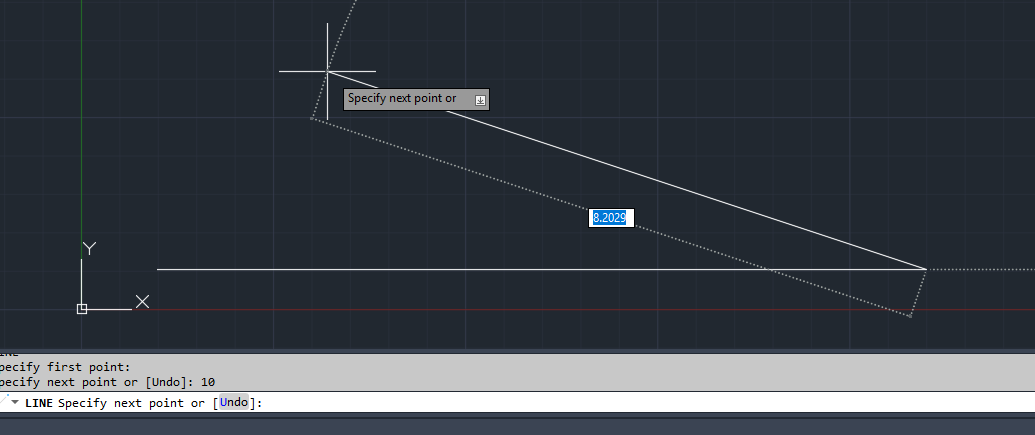
\includegraphics[width=0.5\textwidth]{line_command.png}
              \caption{Line command in AutoCAD Electrical}
          \end{figure}
    \item [\textbf{Significance}] The Line command is essential for creating the basic geometry of electrical drawings, such as wires and cables.
\end{description}

\subsection*{2. Polyline command (PL)}
\addcontentsline{toc}{subsection}{Polyline command (PL)}
\begin{description}
    \item [\textbf{Description}] The Polyline command draws connected line segments and arcs as a single object, useful for complex shapes.
    \item [\textbf{Usage \& Example}] Type "PL" and press Enter. Click to specify points for the polyline segments. Press Enter to complete.
          \begin{figure}[H]
              \centering
              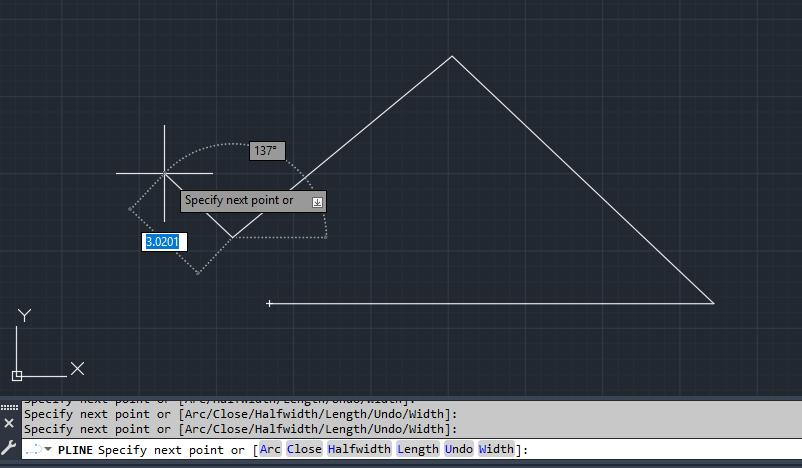
\includegraphics[width=0.5\textwidth]{polyline_command.png}
              \caption{Polyline command in AutoCAD Electrical}
          \end{figure}
    \item [\textbf{Significance}] The Polyline command is essential for creating complex shapes in electrical drawings, allowing continuous lines with multiple segments to be edited as a single object.
\end{description}

\subsection*{3. Circle command (C)}
\addcontentsline{toc}{subsection}{Circle command (C)}
\begin{description}
    \item [\textbf{Description}] Draws circles, commonly used for round components.
    \item [\textbf{Usage \& Example}] Type "C", press Enter, specify center, or drag to desired position, press Enter.
          \begin{figure}[H]
              \centering
              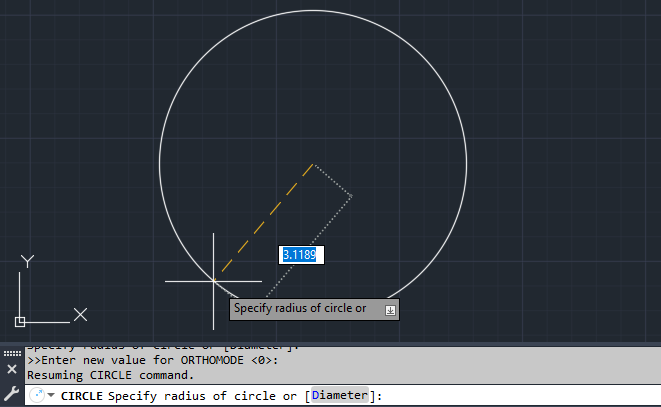
\includegraphics[width=0.5\textwidth]{circle_command.png}
              \caption{Circle command in AutoCAD Electrical}
          \end{figure}
    \item [\textbf{Significance}] Essential for creating round shapes and symbols.
\end{description}

\subsection*{4. Arc command (A)}
\addcontentsline{toc}{subsection}{Arc command (A)}
\begin{description}
    \item [\textbf{Description}] Draws arcs, useful for curved lines.
    \item [\textbf{Usage \& Example}] Type "A", press Enter, specify start, center, and end points.
          \begin{figure}[H]
              \centering
              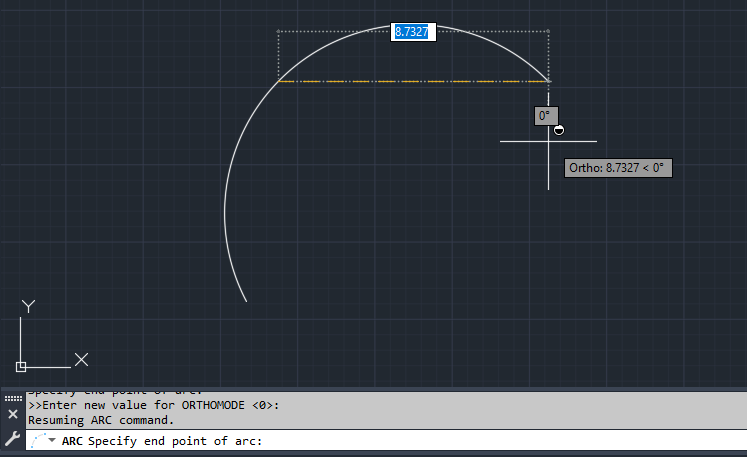
\includegraphics[width=0.5\textwidth]{arc_command.png}
              \caption{Arc command in AutoCAD Electrical}
          \end{figure}
    \item [\textbf{Significance}] Essential for creating curved lines and shapes.
\end{description}

\subsection*{5. Move command (M)}
\addcontentsline{toc}{subsection}{Move command (M)}
\begin{description}
    \item [\textbf{Description}] Moves objects to a new location.
    \item [\textbf{Usage \& Example}] Type "M", press Enter, select object, specify base and destination points.
          \begin{figure}[H]
              \centering
              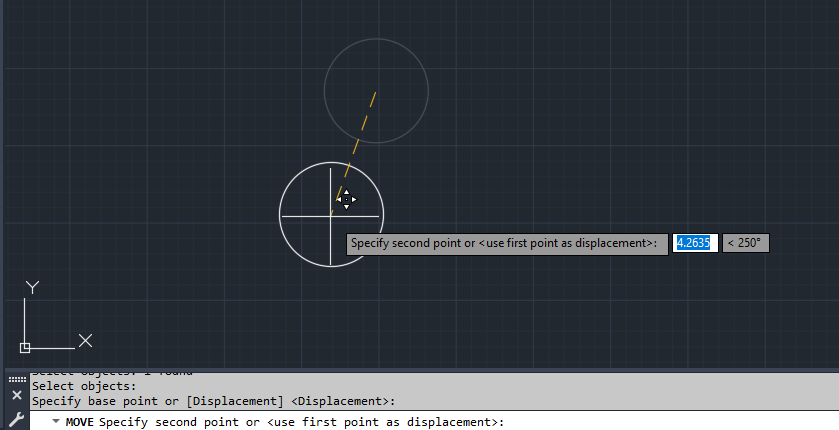
\includegraphics[width=0.5\textwidth]{move_command.png}
              \caption{Move command in AutoCAD Electrical}
          \end{figure}
    \item [\textbf{Significance}] Essential for repositioning objects.
\end{description}

\subsection*{6. Copy command (CO)}
\addcontentsline{toc}{subsection}{Copy command (CO)}
\begin{description}
    \item [\textbf{Description}] Creates copies of objects.
    \item [\textbf{Usage \& Example}] Type "CO", press Enter, select object, specify base and destination points.
          \begin{figure}[H]
              \centering
              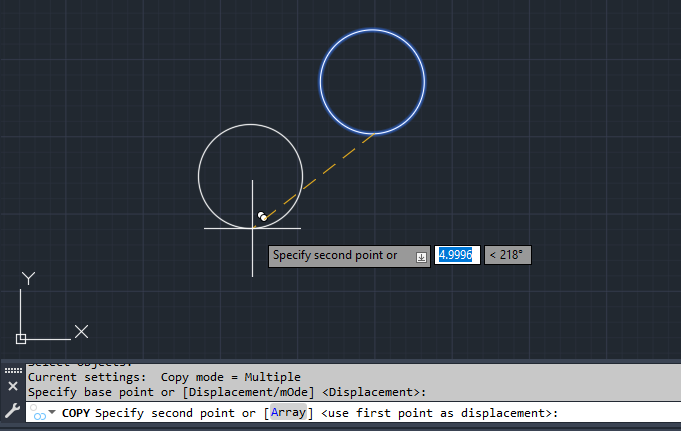
\includegraphics[width=0.5\textwidth]{copy_command.png}
              \caption{Copy command in AutoCAD Electrical}
          \end{figure}
    \item [\textbf{Significance}] Essential for duplicating objects.
\end{description}

\subsection*{7. Rotate command (RO)}
\addcontentsline{toc}{subsection}{Rotate command (RO)}
\begin{description}
    \item [\textbf{Description}] Rotates objects around a base point.
    \item [\textbf{Usage \& Example}] Type "RO", press Enter, select object, specify base point, enter rotation angle.
          \begin{figure}[H]
              \centering
              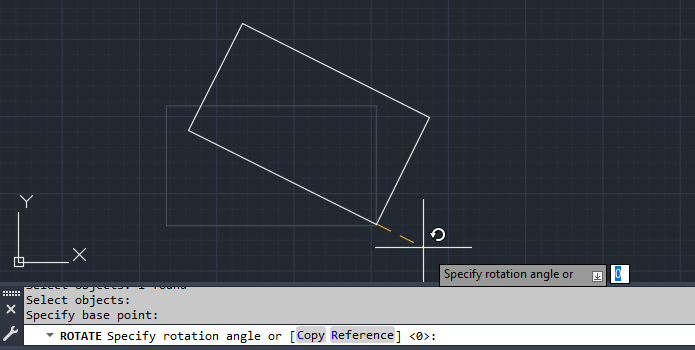
\includegraphics[width=0.5\textwidth]{rotate_command.png}
              \caption{Rotate command in AutoCAD Electrical}
          \end{figure}
    \item [\textbf{Significance}] Essential for changing object orientation.
\end{description}
\subsection*{8. Mirror command (MI)}
\addcontentsline{toc}{subsection}{Mirror command (MI)}
\begin{description}
    \item [\textbf{Description}] Creates a mirrored copy of objects across a specified axis.
    \item [\textbf{Usage \& Example}] Type "MI", press Enter, select object, specify mirror line.
          \begin{figure}[H]
              \centering
              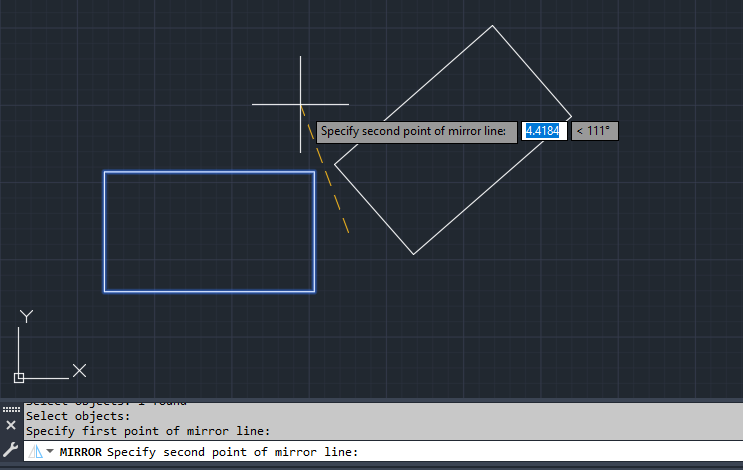
\includegraphics[width=0.5\textwidth]{mirror_command.png}
              \caption{Mirror command in AutoCAD Electrical}
          \end{figure}
    \item [\textbf{Significance}] Useful for symmetrical designs and duplicating components.
\end{description}

\subsection*{9. Extend command (EX)}
\addcontentsline{toc}{subsection}{Extend command (EX)}
\begin{description}
    \item [\textbf{Description}] Extends objects to meet the edges of other objects.
    \item [\textbf{Usage \& Example}] Type "EX", press Enter, select boundary edge, select line to extend.
          \begin{figure}[H]
              \centering
              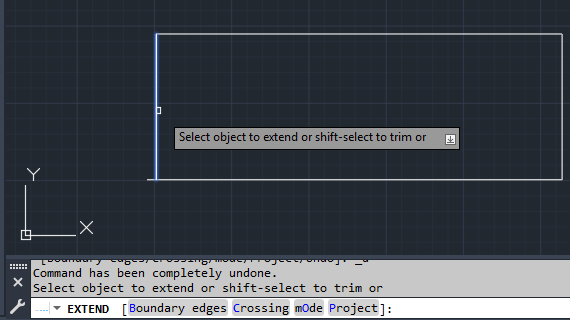
\includegraphics[width=0.5\textwidth]{extend_command.png}
              \caption{Extend command in AutoCAD Electrical}
          \end{figure}
    \item [\textbf{Significance}] Useful for connecting lines and shapes.
\end{description}

\subsection*{10. Trim command (TR)}
\addcontentsline{toc}{subsection}{Trim command (TR)}
\begin{description}
    \item [\textbf{Description}] Trims objects to meet the edges of other objects.
    \item [\textbf{Usage \& Example}] Type "TR", press Enter, select boundary edge, select line to trim.
          \begin{figure}[H]
              \centering
              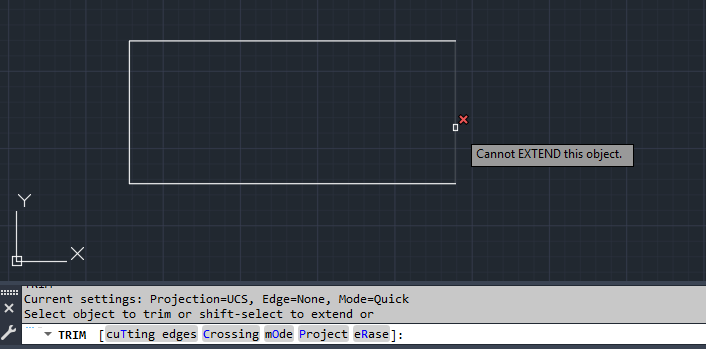
\includegraphics[width=0.5\textwidth]{trim_command.png}
              \caption{Trim command in AutoCAD Electrical}
          \end{figure}
    \item [\textbf{Significance}] Useful for removing unwanted parts of lines and shapes.
\end{description}

\subsection*{11. Erase command (E)}
\addcontentsline{toc}{subsection}{Erase command (E)}
\begin{description}
    \item [\textbf{Description}] Deletes objects from the drawing.
    \item [\textbf{Usage \& Example}] Type "E", press Enter, select object, press Enter to confirm.
          \begin{figure}[H]
              \centering
              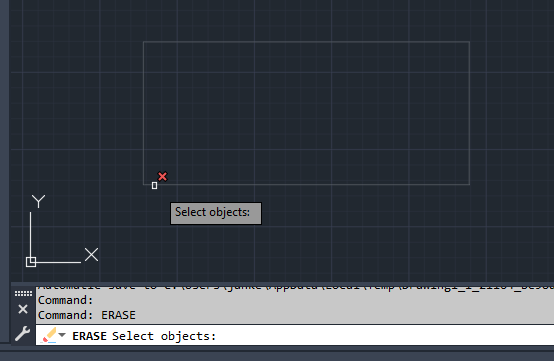
\includegraphics[width=0.5\textwidth]{erase_command.png}
              \caption{Erase command in AutoCAD Electrical}
          \end{figure}
    \item [\textbf{Significance}] Useful for removing unwanted components and symbols.
\end{description}
\subsection*{12. Zoom command (Z)}
\addcontentsline{toc}{subsection}{Zoom command (Z)}
\begin{description}
    \item [\textbf{Description}] Changes the magnification of the drawing view.
    \item [\textbf{Usage \& Example}] Type "Z", press Enter, type "W" for Window, specify corners of the zoom window.
          \begin{figure}[H]
              \centering
              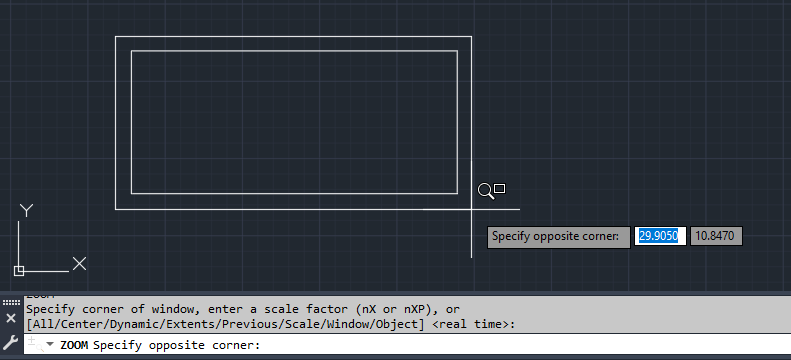
\includegraphics[width=0.5\textwidth]{zoom_command.png}
              \caption{Zoom command in AutoCAD Electrical}
          \end{figure}
    \item [\textbf{Significance}] Essential for focusing on specific areas of the drawing.
\end{description}

\subsection*{13. Layer command (LA)}
\addcontentsline{toc}{subsection}{Layer command (LA)}
\begin{description}
    \item [\textbf{Description}] Manages layers in the drawing.
    \item [\textbf{Usage \& Example}] Type "LA", press Enter, click "New Layer" in Layer Properties Manager, enter layer name.
          \begin{figure}[H]
              \centering
              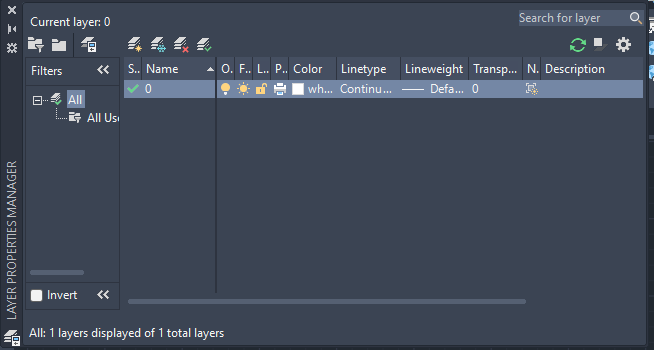
\includegraphics[width=0.5\textwidth]{layer_command.png}
              \caption{Layer command in AutoCAD Electrical}
          \end{figure}
    \item [\textbf{Significance}] Organizes the drawing into different categories.
\end{description}

\subsection*{14. Symbol Insert command (X)}
\addcontentsline{toc}{subsection}{Symbol Insert command (X)}
\begin{description}
    \item [\textbf{Description}] Inserts predefined electrical symbols.
    \item [\textbf{Usage \& Example}] Type "X", press Enter, select symbol from library, specify insertion point.
          \begin{figure}[H]
              \centering
              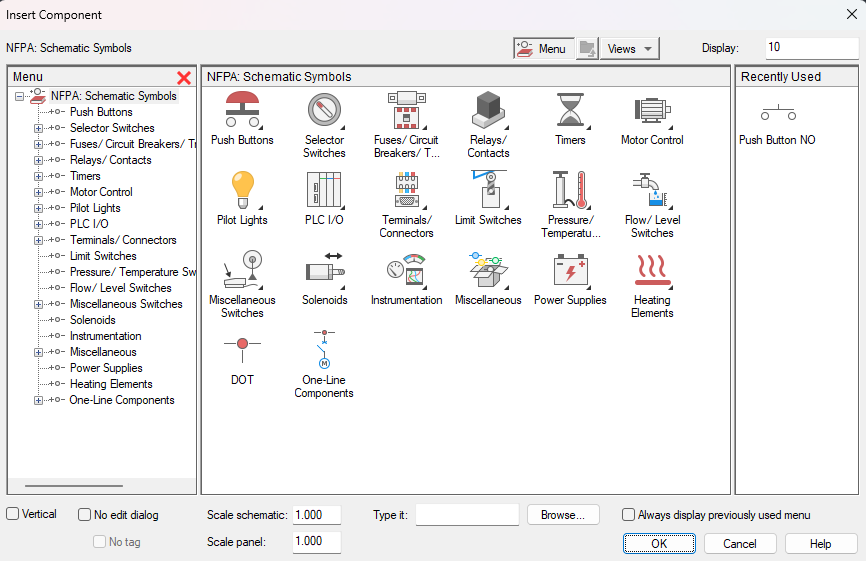
\includegraphics[width=0.5\textwidth]{symbol_insert_command.png}
              \caption{Symbol Insert command in AutoCAD Electrical}
          \end{figure}
    \item [\textbf{Significance}] Adds standard components to the drawing.
\end{description}

\subsection*{15. Wire Number command (W)}
\addcontentsline{toc}{subsection}{Wire Number command (W)}
\begin{description}
    \item [\textbf{Description}] Assigns wire numbers to electrical wires.
    \item [\textbf{Usage \& Example}] Type "W", press Enter, select wire, enter wire number.
          \begin{figure}[H]
              \centering
              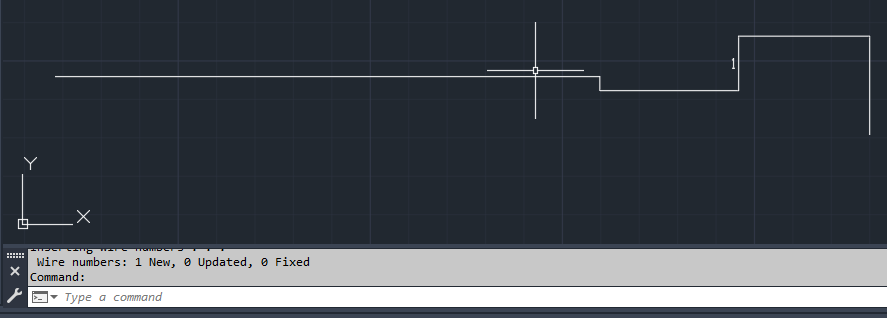
\includegraphics[width=0.5\textwidth]{wire_number_command.png}
              \caption{Wire Number command in AutoCAD Electrical}
          \end{figure}
    \item [\textbf{Significance}] Labels and identifies wires in the drawing.
\end{description}

\subsection*{16. Insert Terminal Strip feature (ITS)}
\addcontentsline{toc}{subsection}{Insert Terminal Strip feature (ITS)}
\begin{description}
    \item [\textbf{Description}] Inserts terminal strips into the drawing.
    \item [\textbf{Usage \& Example}] Type "ITS", press Enter, select terminal strip, specify insertion point.
    \item [\textbf{Significance}] Adds terminal connections accurately.
\end{description}

\subsection*{17. Schematic Tab}
\addcontentsline{toc}{subsection}{Schematic Tab}
\begin{description}
    \item [\textbf{Description}] The Schematic Tab in AutoCAD Electrical provides tools for creating electrical schematics.
    \item [\textbf{Usage \& Example}] Access the Schematic Tab from the ribbon interface. Use the tools within this tab to draw circuit components and connections.
          \begin{figure}[H]
              \centering
              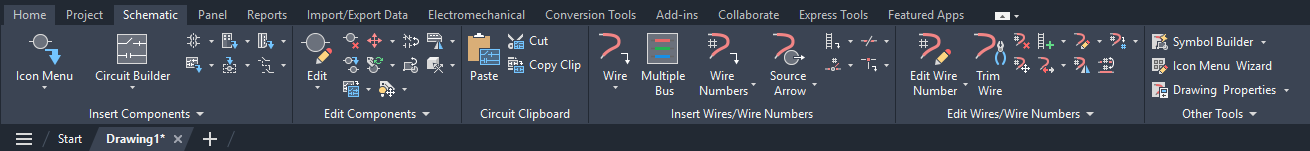
\includegraphics[width=1\textwidth]{create_schematic_command.png}
              \caption{Schematic Tab in AutoCAD Electrical}
          \end{figure}
    \item [\textbf{Significance}] Facilitates the design of detailed electrical circuits with specialized tools.
\end{description}

\subsection*{18. Cross-reference command (XREF)}
\addcontentsline{toc}{subsection}{Cross-reference command (XREF)}
\begin{description}
    \item [\textbf{Description}] Creates cross-references between drawing parts.
    \item [\textbf{Usage \& Example}] Type "XREF", press Enter, select objects, enter reference details.
          \begin{figure}[H]
              \centering
              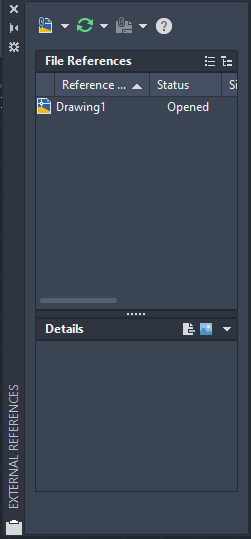
\includegraphics[width=0.3\textwidth]{cross_reference_command.png}
              \caption{Cross-reference command in AutoCAD Electrical}
          \end{figure}
    \item [\textbf{Significance}] Links related components for clarity.
\end{description}

\subsection*{19. AutoNumber feature}
\addcontentsline{toc}{subsection}{AutoNumber feature}
\begin{description}
    \item [\textbf{Description}] Automatically assigns numbers to components.
    \item [\textbf{Usage \& Example}] Type "AN", press Enter, select components, specify options.
    \item [\textbf{Significance}] Ensures consistent and accurate numbering.
\end{description}

\subsection*{20. PLC Wiring feature}
\addcontentsline{toc}{subsection}{PLC Wiring feature}
\begin{description}
    \item [\textbf{Description}] Creates wiring diagrams for PLCs.
    \item [\textbf{Usage \& Example}] Type "PLC", press Enter, draw PLC components and connections.
    \item [\textbf{Significance}] Essential for designing PLC circuits.
\end{description}

\subsection*{21. Component Tagging feature}
\addcontentsline{toc}{subsection}{Component Tagging feature}
\begin{description}
    \item [\textbf{Description}] Assigns tags to electrical components.
    \item [\textbf{Usage \& Example}] Type "CT", press Enter, select component, enter tag details.
    \item [\textbf{Significance}] Helps in identifying and labeling components.
\end{description}

\subsection*{22. Project Management feature}
\addcontentsline{toc}{subsection}{Project Management feature}
\begin{description}
    \item [\textbf{Description}] Manages electrical projects, organizing and controlling project files.
    \item [\textbf{Usage \& Example}] Type "PE", press Enter, click "New Project" in Project Manager, enter details.
    \item [\textbf{Significance}] Essential for organizing and managing project files and settings.
\end{description}

\subsection*{23. Block Editor command (BEDIT)}
\addcontentsline{toc}{subsection}{Block Editor command (BEDIT)}
\begin{description}
    \item [\textbf{Description}] Creates and edits blocks, defining reusable components.
    \item [\textbf{Usage \& Example}] Type "BEDIT", press Enter, draw components in Block Editor, save block.
          \begin{figure}[H]
              \centering
              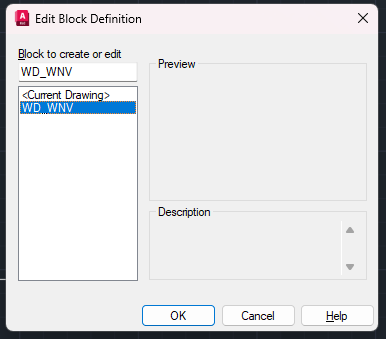
\includegraphics[width=0.5\textwidth]{block_editor_command.png}
              \caption{Block Editor command in AutoCAD Electrical}
          \end{figure}
    \item [\textbf{Significance}] Essential for creating reusable components for consistent use.
\end{description}

\section*{Discussion \& Conclusion}
\addcontentsline{toc}{section}{Discussion \& Conclusion}
This report explored essential AutoCAD Electrical commands for creating and modifying electrical drawings. Commands like Line, Polyline, Circle, and Arc are fundamental, while Move, Copy, Rotate, and Mirror aid in editing. Layer and Symbol Insert commands help organize drawings, and Wire Number and Component Tagging enhance clarity. Mastering these commands improves productivity and ensures accurate designs. AutoCAD Electrical's comprehensive tools streamline the design process, improving workflow and project outcomes.

% \bibliographystyle{IEEEtran}
% \renewcommand{\bibname}{References}
% \addcontentsline{toc}{section}{References}
% \bibliography{ref}

\end{document}
